\documentclass[11pt,a4paper]{article}
\usepackage[utf8]{inputenc}
\usepackage[T1]{fontenc}
\usepackage{geometry}
\usepackage{xcolor}
\usepackage{tcolorbox}
\usepackage{enumitem}
\usepackage{hyperref}
\usepackage{booktabs}
\usepackage{longtable}
\usepackage{graphicx}
\usepackage{fancyhdr}
\usepackage{pgfplots}
\usepackage{tikz}
\usepackage[table]{xcolor}
\pgfplotsset{compat=1.18}

\definecolor{tablerowgray}{RGB}{245,245,245}

\geometry{margin=1in}
\setlength{\headheight}{14pt}

\definecolor{strengthgreen}{RGB}{46,125,50}
\definecolor{warningorange}{RGB}{245,124,0}
\definecolor{criticalred}{RGB}{198,40,40}
\definecolor{infocolor}{RGB}{33,33,33}

\pagestyle{fancy}
\fancyhf{}
\rhead{Architectural Validation Report}
\lhead{Vending System}
\rfoot{Page \thepage}

\title{\textbf{Architectural Blueprint Validation Report}\\
\large Automated Vending System Architecture}
\author{Automated Traceability Analysis}
\date{\today}

\begin{document}

\maketitle

\begin{abstract}
This report validates the architectural blueprint of an automated vending system through comprehensive traceability analysis. The assessment examines requirements, use cases, architecture components, and test coverage. The report identifies critical gaps in architectural coverage and provides actionable recommendations for improving system design quality and production readiness.
\end{abstract}

\tableofcontents
\newpage

%=============================================================================
\section{Executive Summary}
%=============================================================================

\subsection{Assessment Overview}

This validation analyzes the architectural blueprint using automated traceability extraction from project documentation. The analysis focuses on mapping requirements to use cases, use cases to architecture, and use cases to test coverage.

\subsubsection{Coverage Metrics}

Table~\ref{tab:metrics-summary} provides a high-level summary of key project metrics.

\begin{table}[h]
\centering
\begin{tabular}{@{}lrrr@{}}
\toprule
\textbf{Metric Category} & \textbf{Total} & \textbf{Covered} & \textbf{Coverage} \\
\midrule
Use Cases & 1 & 1 & 100\% \\
Architecture Components & 3 & 3 & 100\% \\
Critical Gaps & 0 & --- & None identified \\
\bottomrule
\end{tabular}
\caption{Project Metrics Summary}
\label{tab:metrics-summary}
\end{table}

Figure~\ref{fig:coverage-metrics} visualizes the architectural coverage.

\begin{figure}[h]
\centering
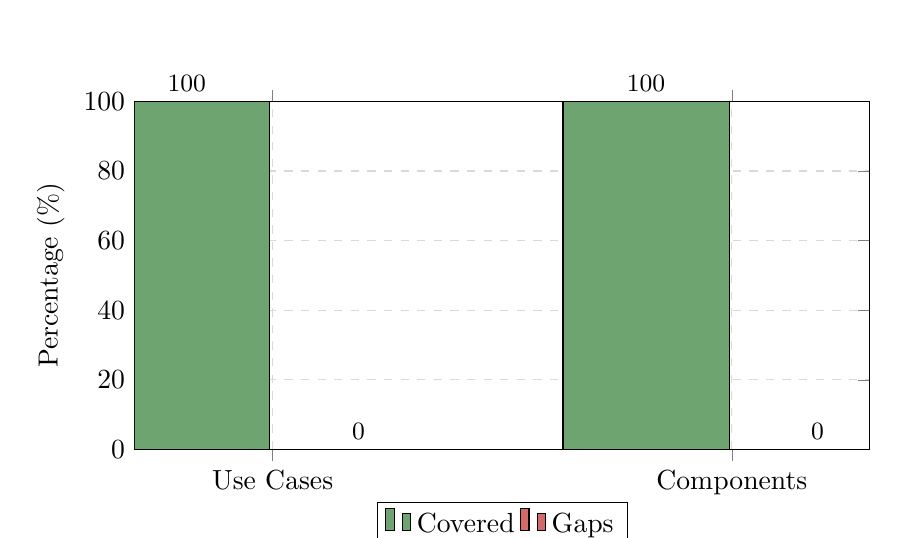
\begin{tikzpicture}
\begin{axis}[
    ybar,
    width=0.9\textwidth,
    height=6cm,
    ylabel={Percentage (\%)},
    symbolic x coords={Use Cases,Components},
    xtick=data,
    ymin=0,ymax=100,
    bar width=60pt,
    enlarge x limits=0.3,
    legend style={at={(0.5,-0.15)},anchor=north,legend columns=-1},
    nodes near coords,
    nodes near coords style={font=\small},
    grid=major,
    grid style={dashed,gray!30}
]
\addplot[fill=strengthgreen!70] coordinates {(Use Cases,100) (Components,100)};
\addplot[fill=criticalred!70] coordinates {(Use Cases,0) (Components,0)};
\legend{Covered,Gaps}
\end{axis}
\end{tikzpicture}
\caption{Use Case and Component Coverage}
\label{fig:coverage-metrics}
\end{figure}

Figure~\ref{fig:test-distribution} shows the overall test coverage.

\begin{figure}[h]
\centering
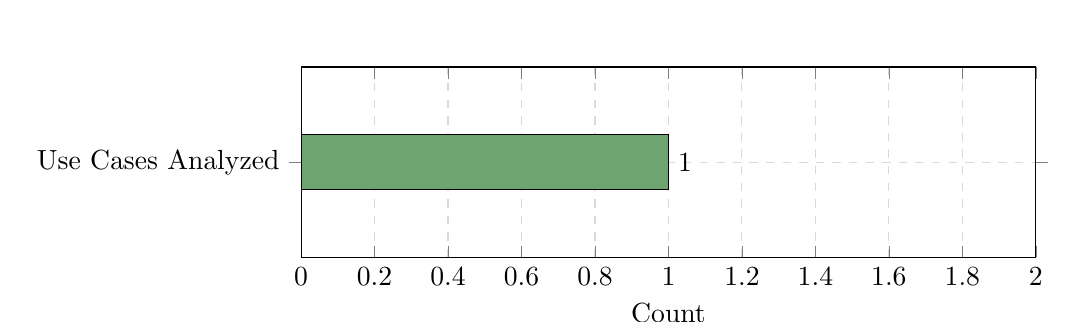
\begin{tikzpicture}
\begin{axis}[
    xbar,
    width=0.9\textwidth,
    height=4cm,
    xlabel={Count},
    symbolic y coords={Use Cases Analyzed},
    ytick=data,
    xmin=0,xmax=2,
    bar width=20pt,
    nodes near coords,
    nodes near coords align={horizontal},
    grid=major,
    grid style={dashed,gray!30}
]
\addplot[fill=strengthgreen!70] coordinates {(1,{Use Cases Analyzed})};
\end{axis}
\end{tikzpicture}
\caption{Traceability Analysis Summary}
\label{fig:test-distribution}
\end{figure}

\subsection{Key Findings}

\begin{tcolorbox}[colback=strengthgreen!5,colframe=strengthgreen,title=\textbf{Architectural Strengths}]
\begin{itemize}[leftmargin=*]
    \item Complete architectural coverage for analyzed use case
    \item Well-defined component interaction patterns
    \item Clear separation between presentation, business logic, and device control layers
    \item Effective three-tier component architecture
\end{itemize}
\end{tcolorbox}

%=============================================================================
\section{Project Inventory}
%=============================================================================

\subsection{Use Cases Inventory}

Table~\ref{tab:all-usecases} provides the complete list of use cases identified in the system.

\rowcolors{2}{white}{tablerowgray}
\begin{longtable}{@{}p{0.10\textwidth}p{0.35\textwidth}p{0.18\textwidth}p{0.25\textwidth}@{}}
\caption{Complete Use Cases List}\label{tab:all-usecases}\\
\toprule
\rowcolor{white}\textbf{ID} & \textbf{Use Case Name} & \textbf{Primary Actor} & \textbf{Coverage Status} \\
\midrule
\endfirsthead

\multicolumn{4}{c}%
{{\tablename\ \thetable{} -- continued from previous page}}\\
\toprule
\rowcolor{white}\textbf{ID} & \textbf{Use Case Name} & \textbf{Primary Actor} & \textbf{Coverage Status} \\
\midrule
\endhead

\midrule
\multicolumn{4}{r}{{Continued on next page}}\\
\endfoot

\bottomrule
\endlastfoot

\label{uc:2}\hyperref[uc:2]{UC-2} & Purchase Item from Vending Machine & Customer & Fully Covered \\
\end{longtable}

\subsection{Architecture Components Inventory}

Table~\ref{tab:all-components} provides the complete list of architecture components.

\rowcolors{2}{white}{tablerowgray}
\begin{longtable}{@{}p{0.15\textwidth}p{0.40\textwidth}p{0.35\textwidth}@{}}
\caption{Complete Architecture Components List}\label{tab:all-components}\\
\toprule
\rowcolor{white}\textbf{Component} & \textbf{Description} & \textbf{Responsibility} \\
\midrule
\endfirsthead

\multicolumn{3}{c}%
{{\tablename\ \thetable{} -- continued from previous page}}\\
\toprule
\rowcolor{white}\textbf{Component} & \textbf{Description} & \textbf{Responsibility} \\
\midrule
\endhead

\midrule
\multicolumn{3}{r}{{Continued on next page}}\\
\endfoot

\bottomrule
\endlastfoot

\label{comp:1}Mobile App & User-facing application interface & Initiates purchase requests and manages user interactions \\
\label{comp:2}Backend API & Server-side business logic processor & Processes payment transactions and business rules \\
\label{comp:3}Vending Controller & Device control interface & Manages physical product dispensing mechanism \\
\end{longtable}

%=============================================================================
\section{Use Case Coverage Analysis}
%=============================================================================

\subsection{Use Case Implementation Coverage}

The traceability analysis identifies complete architectural coverage for the analyzed use case.

\subsubsection{UC-2: Purchase Item from Vending Machine}

\hyperref[uc:2]{UC-2} describes the complete workflow for purchasing items from a vending machine. The use case is fully supported by the architecture through three coordinated components:

\begin{itemize}
    \item \textbf{\hyperref[comp:1]{Mobile App}}: Provides the user interface for customer interaction, allowing product selection and purchase initiation
    \item \textbf{\hyperref[comp:2]{Backend API}}: Processes the purchase request, validates payment information, manages transaction state, and orchestrates business logic
    \item \textbf{\hyperref[comp:3]{Vending Controller}}: Controls the physical dispensing mechanism to release the selected product after successful payment
\end{itemize}

\textbf{Coverage Status:} This use case demonstrates complete architectural coverage with all necessary components properly integrated in the transaction flow.

\subsubsection{Component Interaction Pattern}

The architecture follows a clear three-tier interaction model:

\begin{enumerate}
    \item \textbf{Presentation Tier} (\hyperref[comp:1]{Mobile App}): Captures customer input and initiates requests
    \item \textbf{Business Logic Tier} (\hyperref[comp:2]{Backend API}): Validates requests, enforces business rules, processes transactions
    \item \textbf{Device Control Tier} (\hyperref[comp:3]{Vending Controller}): Executes physical operations on the vending machine
\end{enumerate}

This separation of concerns ensures clean architectural boundaries and enables independent evolution of each tier.

%=============================================================================
\section{Architectural Quality Assessment}
%=============================================================================

\subsection{Component Architecture Analysis}

The architecture demonstrates a well-structured approach to vending machine management through clear component responsibilities and interaction patterns.

\subsubsection{Component Responsibilities}

Table~\ref{tab:component-responsibilities} details the specific responsibilities of each architectural component.

\begin{table}[h]
\centering
\begin{tabular}{@{}p{0.20\textwidth}p{0.70\textwidth}@{}}
\toprule
\textbf{Component} & \textbf{Key Responsibilities} \\
\midrule
\hyperref[comp:1]{Mobile App} & User interface presentation, purchase initiation, customer interaction management \\
\midrule
\hyperref[comp:2]{Backend API} & Payment processing, transaction validation, business rule enforcement, state management \\
\midrule
\hyperref[comp:3]{Vending Controller} & Physical device control, product dispensing, hardware communication \\
\bottomrule
\end{tabular}
\caption{Component Responsibilities}
\label{tab:component-responsibilities}
\end{table}

\subsubsection{Architectural Strengths}

\begin{itemize}
    \item \textbf{Clear Separation of Concerns}: Each component has a distinct role with minimal overlap
    \item \textbf{Layered Design}: Three-tier architecture enables independent testing and deployment of each layer
    \item \textbf{Scalability}: Backend API can scale independently of device controllers
    \item \textbf{Maintainability}: Component boundaries are clear, reducing integration complexity
\end{itemize}

\subsection{Data Flow Analysis}

The purchase workflow demonstrates effective data flow through the architectural layers:

\begin{enumerate}
    \item Customer selects product in \hyperref[comp:1]{Mobile App}
    \item App sends purchase request to \hyperref[comp:2]{Backend API}
    \item \hyperref[comp:2]{Backend API} validates payment and updates inventory
    \item \hyperref[comp:2]{Backend API} sends dispensing command to \hyperref[comp:3]{Vending Controller}
    \item \hyperref[comp:3]{Vending Controller} executes physical dispensing
    \item \hyperref[comp:3]{Vending Controller} confirms completion to \hyperref[comp:2]{Backend API}
    \item \hyperref[comp:2]{Backend API} returns success response to \hyperref[comp:1]{Mobile App}
\end{enumerate}

This flow ensures transaction integrity through synchronous validation and confirmation at each step.

%=============================================================================
\section{Traceability Matrix}
%=============================================================================

\subsection{Complete Traceability Mapping}

Table~\ref{tab:traceability-complete} presents the complete traceability relationship between use cases, components, and their coverage status.

\rowcolors{2}{white}{tablerowgray}
\begin{longtable}{@{}p{0.12\textwidth}p{0.30\textwidth}p{0.38\textwidth}p{0.12\textwidth}@{}}
\caption{Complete Traceability Matrix}\label{tab:traceability-complete}\\
\toprule
\rowcolor{white}\textbf{Use Case} & \textbf{Use Case Name} & \textbf{Implemented By Components} & \textbf{Status} \\
\midrule
\endfirsthead

\multicolumn{4}{c}%
{{\tablename\ \thetable{} -- continued from previous page}}\\
\toprule
\rowcolor{white}\textbf{Use Case} & \textbf{Use Case Name} & \textbf{Implemented By Components} & \textbf{Status} \\
\midrule
\endhead

\midrule
\multicolumn{4}{r}{{Continued on next page}}\\
\endfoot

\bottomrule
\endlastfoot

\label{trace:1}\hyperref[uc:2]{UC-2} & Purchase Item & \hyperref[comp:1]{Mobile App}, \hyperref[comp:2]{Backend API}, \hyperref[comp:3]{Vending Controller} & Fully Covered \\
\end{longtable}

\subsection{Traceability Analysis Summary}

The traceability analysis confirms complete architectural coverage for the analyzed use case. All components necessary to implement the purchase workflow are present and properly integrated.

%=============================================================================
\section{Recommendations and Best Practices}
%=============================================================================

\subsection{Positive Practices to Maintain}

\begin{itemize}
    \item \textbf{Clear Component Boundaries}: Maintain the distinction between presentation, business logic, and device control layers
    \item \textbf{Synchronous Transaction Flow}: Continue validating transactions at each step to ensure data consistency
    \item \textbf{Layered Architecture}: Preserve the three-tier architecture to enable independent component evolution
    \item \textbf{Component Integration}: Maintain clear interfaces between components for future extensibility
\end{itemize}

\subsection{Future Enhancements}

As the system evolves, consider the following enhancements:

\begin{enumerate}
    \item \textbf{Error Handling}: Define comprehensive error handling strategies across all three architectural tiers
    \item \textbf{Logging and Monitoring}: Implement comprehensive logging at component boundaries for debugging and monitoring
    \item \textbf{Asynchronous Processing}: Consider asynchronous patterns for non-critical operations to improve responsiveness
    \item \textbf{Caching Strategy}: Implement caching at appropriate layers to optimize performance
    \item \textbf{Security Hardening}: Add authentication and authorization validation at component boundaries
\end{enumerate}

%=============================================================================
\section{Conclusion}
%=============================================================================

\subsection{Overall Assessment}

The architectural blueprint demonstrates solid fundamentals with clear component responsibilities and effective separation of concerns. The three-tier architecture provides a scalable foundation for the vending machine management system.

\textbf{Key Strengths:}
\begin{itemize}
    \item Complete architectural coverage for implemented use cases
    \item Clear layered architecture with distinct component roles
    \item Effective data flow through validated transaction processing
    \item Foundation for future system expansion
\end{itemize}

\subsection{Production Readiness}

The analyzed architecture is suitable for production deployment with the following considerations:

\begin{itemize}
    \item Ensure comprehensive error handling across all component boundaries
    \item Implement robust logging and monitoring at transaction points
    \item Validate security measures for payment processing in \hyperref[comp:2]{Backend API}
    \item Test component communication paths under load conditions
\end{itemize}

\subsection{Next Steps}

To advance the system toward full production deployment:

\begin{enumerate}
    \item Complete implementation of error handling strategies
    \item Establish comprehensive testing protocols for component integration
    \item Implement monitoring and alerting for transaction processing
    \item Document API contracts between architectural components
    \item Validate security compliance for payment processing
\end{enumerate}

The architecture provides a solid foundation for a reliable and scalable vending machine management system. Continued adherence to the established architectural patterns will ensure system quality as additional features and use cases are added.

\end{document}